\subsection{Calculator}
In the chatbot there has been implemented a simple calculator. The simple calculator is made using NCalc, Ncalc is a mathematical expressions evaluator in .NET [\ref{subsec:Csharp}]. NCalc is made so that it parses any expression and evaluate the result given, this is including static or dynamic parameter and custom functions. NCalc  allows expression evaluation because NCalc is a set of assemblies which allows texpression evaluation. The main class NCalc make use of is Expression.  This class has a method Evaluate() returning the actual value of its String representation. \cite{Ncalc}

\noindent Define parameters, even dynamic or expressions
\begin{figure}[H]
    \centering
    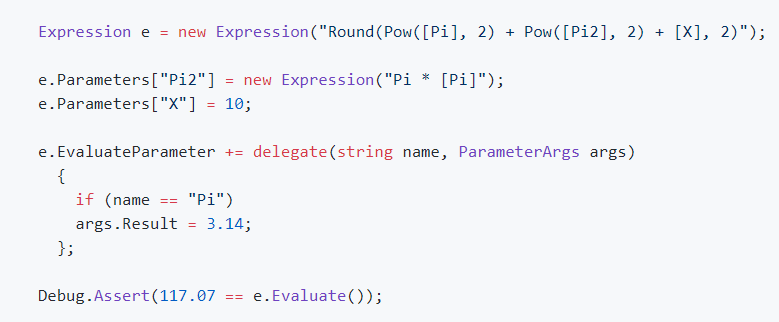
\includegraphics[width=0.6\textwidth]{figures/NCalc.png}
    \caption{The code for define parameters, even dynamic or expressions}
    \label{fig:NCalc}
\end{figure}


